\documentclass[11pt]{article}

\usepackage[margin=1in]{geometry}
\usepackage{amsmath,amssymb,mathtools}
\usepackage{booktabs}
\usepackage{graphicx}
\usepackage{float}

\setlength{\parindent}{0pt}
\setlength{\parskip}{0.55em}
\renewcommand{\arraystretch}{1.18}

\newcommand{\ii}{\mathrm{i}}
\newcommand{\eoc}{\mathrm{EOC}}
\newcommand{\norm}[1]{\left\lVert #1\right\rVert}

\title{Von Neumann Stability Handout\\
Finite Difference Methods for $u_t+a u_x=0$}
\author{Rishabh Kumar}
\date{\today}

\begin{document}
\maketitle

\section{Fourier-Mode Test}

For the linear advection equation
\begin{equation}
    u_t+a u_x=0,\qquad a>0,
\end{equation}
write
\begin{equation}
    \nu=\frac{ak}{h}.
\end{equation}
Von Neumann stability is tested by inserting
\begin{equation}
    v_m^n=G^n e^{\ii m\theta}
\end{equation}
into the finite difference scheme.  The method is stable if
\begin{equation}
    |G(\theta)|\le 1
    \qquad\text{for all }\theta.
\end{equation}

\section{Norms Used in the Numerical Evidence}

At the final time $T=t_N$, define the grid error
\begin{equation}
    e_m^N=v_m^N-u(x_m,T).
\end{equation}
The convergence and sweep plots use the discrete norms
\begin{align}
    E_1
    &=
    h\sum_m |e_m^N|,
    \\
    E_2
    &=
    \left(h\sum_m |e_m^N|^2\right)^{1/2},
    \\
    E_\infty
    &=
    \max_m |e_m^N|.
\end{align}
The first two approximate the continuous $L^1$ and $L^2$ norms:
\begin{equation}
    E_1\approx \norm{e(\cdot,T)}_{L^1},
    \qquad
    E_2\approx \norm{e(\cdot,T)}_{L^2}.
\end{equation}
The maximum norm $E_\infty$ records the largest pointwise error anywhere on the grid.
It is therefore the most sensitive norm to a localized overshoot, undershoot, or
oscillation.

The experimental order of convergence is computed by comparing errors on two
successive meshes:
\begin{equation}
    \eoc
    =
    \frac{\log(E_h/E_{h/2})}{\log 2}.
\end{equation}
If $E_h\approx C h^p$, then $\eoc\approx p$.

For the $\lambda$-stability sweep, one also monitors
\begin{equation}
    \norm{v^N}_\infty=\max_m |v_m^N|.
\end{equation}
This is not an error norm; it is a final-time amplitude.  Since the exact solution is
bounded by $1$, very large values of $\norm{v^N}_\infty$ indicate nonphysical growth
and hence numerical instability.

\section{Explicit Schemes}

\subsection{FTFS}

The scheme is
\begin{equation}
    v_m^{n+1}=v_m^n-\nu(v_{m+1}^n-v_m^n).
\end{equation}
Substituting $v_m^n=G^n e^{\ii m\theta}$ gives
\begin{equation}
    G=1-\nu(e^{\ii\theta}-1)
    =
    1+\nu-\nu e^{\ii\theta}.
\end{equation}
Thus
\begin{align}
    |G|^2
    &=
    (1+\nu-\nu\cos\theta)^2+\nu^2\sin^2\theta\\
    &=
    1+2\nu(1+\nu)(1-\cos\theta).
\end{align}
For $\nu>0$ and $\theta\ne0$, $|G|>1$.  FTFS is unstable for right-moving advection.

\subsection{FTBS}

The scheme is
\begin{equation}
    v_m^{n+1}=v_m^n-\nu(v_m^n-v_{m-1}^n).
\end{equation}
Then
\begin{equation}
    G=1-\nu(1-e^{-\ii\theta})
    =
    1-\nu+\nu e^{-\ii\theta}.
\end{equation}
Therefore
\begin{align}
    |G|^2
    &=
    (1-\nu+\nu\cos\theta)^2+\nu^2\sin^2\theta\\
    &=
    1-2\nu(1-\nu)(1-\cos\theta).
\end{align}
For all $\theta$,
\begin{equation}
    |G|\le1
    \quad\Longleftrightarrow\quad
    0\le\nu\le1.
\end{equation}
This is the usual upwind CFL condition.

\subsection{FTCS}

The scheme is
\begin{equation}
    v_m^{n+1}=v_m^n-\frac{\nu}{2}(v_{m+1}^n-v_{m-1}^n).
\end{equation}
Hence
\begin{equation}
    G=1-\frac{\nu}{2}(e^{\ii\theta}-e^{-\ii\theta})
    =
    1-\ii\nu\sin\theta.
\end{equation}
Consequently
\begin{equation}
    |G|^2=1+\nu^2\sin^2\theta.
\end{equation}
For every nonzero $\nu$, some Fourier modes satisfy $|G|>1$.  FTCS is unstable.

\subsection{CTCS or Leapfrog}

The scheme is
\begin{equation}
    v_m^{n+1}=v_m^{n-1}-\nu(v_{m+1}^n-v_{m-1}^n).
\end{equation}
Substituting a Fourier mode gives
\begin{equation}
    G-G^{-1}=-\nu(e^{\ii\theta}-e^{-\ii\theta})
    =
    -2\ii\nu\sin\theta.
\end{equation}
Multiplying by $G$,
\begin{equation}
    G^2+2\ii\nu\sin\theta\,G-1=0.
\end{equation}
The roots are
\begin{equation}
    G=-\ii\nu\sin\theta
    \pm \sqrt{1-\nu^2\sin^2\theta}.
\end{equation}
For the square root to be real for all $\theta$, we need
\begin{equation}
    |\nu|\le1.
\end{equation}
When this holds, the two roots lie on the unit circle.  Leapfrog is therefore stable under $|\nu|\le1$, but it has a computational mode and needs a stable startup step.

\subsection{Lax--Friedrichs}

The scheme is
\begin{equation}
    v_m^{n+1}
    =
    \frac12(v_{m+1}^n+v_{m-1}^n)
    -\frac{\nu}{2}(v_{m+1}^n-v_{m-1}^n).
\end{equation}
Thus
\begin{align}
    G
    &=
    \frac12(e^{\ii\theta}+e^{-\ii\theta})
    -\frac{\nu}{2}(e^{\ii\theta}-e^{-\ii\theta})\\
    &=
    \cos\theta-\ii\nu\sin\theta.
\end{align}
Therefore
\begin{equation}
    |G|^2
    =
    \cos^2\theta+\nu^2\sin^2\theta
    =
    1-(1-\nu^2)\sin^2\theta.
\end{equation}
The stability condition is
\begin{equation}
    |\nu|\le1.
\end{equation}

\subsection{Lax--Wendroff}

The scheme is
\begin{equation}
    v_m^{n+1}
    =
    v_m^n
    -\frac{\nu}{2}(v_{m+1}^n-v_{m-1}^n)
    +\frac{\nu^2}{2}(v_{m+1}^n-2v_m^n+v_{m-1}^n).
\end{equation}
The amplification factor is
\begin{equation}
    G=
    1-\ii\nu\sin\theta+\nu^2(\cos\theta-1).
\end{equation}
Let $s=\sin(\theta/2)$.  Then
\begin{equation}
    \cos\theta-1=-2s^2,
    \qquad
    \sin^2\theta=4s^2(1-s^2).
\end{equation}
Therefore
\begin{align}
    |G|^2
    &=
    (1-2\nu^2s^2)^2+4\nu^2s^2(1-s^2)\\
    &=
    1-4\nu^2(1-\nu^2)s^4.
\end{align}
Hence
\begin{equation}
    |G|\le1\quad \text{for all }\theta
    \quad\Longleftrightarrow\quad
    |\nu|\le1.
\end{equation}

\subsection{Beam--Warming}

For $a>0$, the Beam--Warming scheme is
\begin{equation}
    v_m^{n+1}
    =
    v_m^n
    -\frac{\nu}{2}(3v_m^n-4v_{m-1}^n+v_{m-2}^n)
    +\frac{\nu^2}{2}(v_m^n-2v_{m-1}^n+v_{m-2}^n).
\end{equation}
Let $q=e^{-\ii\theta}$.  Then
\begin{equation}
    G=
    1-\frac{\nu}{2}(3-4q+q^2)
    +\frac{\nu^2}{2}(1-2q+q^2).
\end{equation}
Set $\delta=1-q$.  Since
\begin{equation}
    3-4q+q^2=2\delta+\delta^2,
    \qquad
    1-2q+q^2=\delta^2,
\end{equation}
we get
\begin{equation}
    G=1-\nu\delta+\frac{\nu(\nu-1)}{2}\delta^2.
\end{equation}
Using
\begin{equation}
    \delta+\overline{\delta}=|\delta|^2
    =
    4\sin^2(\theta/2),
\end{equation}
one obtains
\begin{equation}
    |G|^2
    =
    1-4\nu(2-\nu)(1-\nu)^2\sin^4(\theta/2).
\end{equation}
Thus
\begin{equation}
    |G|\le1\quad\text{for all }\theta
    \quad\Longleftrightarrow\quad
    0\le\nu\le2.
\end{equation}

\section{Implicit Schemes}

\subsection{BTFS}

BTFS is
\begin{equation}
    v_m^{n+1}
    +\nu(v_{m+1}^{n+1}-v_m^{n+1})=v_m^n.
\end{equation}
Thus
\begin{equation}
    G\left[1+\nu(e^{\ii\theta}-1)\right]=1,
\end{equation}
so
\begin{equation}
    G=\frac{1}{1-\nu+\nu e^{\ii\theta}}.
\end{equation}
The denominator satisfies
\begin{equation}
    |1-\nu+\nu e^{\ii\theta}|^2
    =
    1-2\nu(1-\nu)(1-\cos\theta).
\end{equation}
For $0<\nu<1$, this can be smaller than $1$, so $|G|>1$ for some modes.  For $\nu\ge1$, the denominator modulus is at least $1$.  BTFS is therefore not the natural stable implicit upwind scheme for $a>0$ when $0<\nu<1$.

\subsection{BTBS}

BTBS is
\begin{equation}
    v_m^{n+1}
    +\nu(v_m^{n+1}-v_{m-1}^{n+1})=v_m^n.
\end{equation}
Then
\begin{equation}
    G\left[1+\nu-\nu e^{-\ii\theta}\right]=1,
\end{equation}
and
\begin{equation}
    G=\frac{1}{1+\nu-\nu e^{-\ii\theta}}.
\end{equation}
The denominator has modulus squared
\begin{equation}
    |1+\nu-\nu e^{-\ii\theta}|^2
    =
    1+2\nu(1+\nu)(1-\cos\theta)\ge1.
\end{equation}
Hence
\begin{equation}
    |G|\le1
    \qquad\text{for all }\nu\ge0.
\end{equation}
BTBS is unconditionally stable for right-moving advection.

\subsection{BTCS}

BTCS is
\begin{equation}
    v_m^{n+1}
    +\frac{\nu}{2}(v_{m+1}^{n+1}-v_{m-1}^{n+1})=v_m^n.
\end{equation}
Therefore
\begin{equation}
    G\left[1+\frac{\nu}{2}(e^{\ii\theta}-e^{-\ii\theta})\right]=1,
\end{equation}
or
\begin{equation}
    G=\frac{1}{1+\ii\nu\sin\theta}.
\end{equation}
Thus
\begin{equation}
    |G|^2=\frac{1}{1+\nu^2\sin^2\theta}\le1.
\end{equation}
BTCS is unconditionally stable in the von Neumann sense.

\subsection{Crank--Nicolson}

Crank--Nicolson is
\begin{equation}
    v_m^{n+1}
    +\frac{\nu}{4}(v_{m+1}^{n+1}-v_{m-1}^{n+1})
    =
    v_m^n
    -\frac{\nu}{4}(v_{m+1}^{n}-v_{m-1}^{n}).
\end{equation}
Substitution gives
\begin{equation}
    G\left[1+\frac{\ii\nu}{2}\sin\theta\right]
    =
    1-\frac{\ii\nu}{2}\sin\theta.
\end{equation}
Hence
\begin{equation}
    G=
    \frac{1-\frac{\ii\nu}{2}\sin\theta}
         {1+\frac{\ii\nu}{2}\sin\theta}.
\end{equation}
The numerator and denominator are complex conjugates, so
\begin{equation}
    |G|=1.
\end{equation}
Crank--Nicolson is neutrally stable for all $\nu$.

\section{Interpreting the $\lambda$ Parameter Sweeps}

The numerical parameter sweep in the Beamer slides is a direct computational test of
the stability conditions derived above.  In the assignment problem the equation is
\begin{equation}
    u_t+u_x=0,
\end{equation}
so the wave speed is $a=1$.  Therefore
\begin{equation}
    \nu=\frac{ak}{h}=\frac{k}{h}=\lambda.
\end{equation}
Thus the parameter $\lambda$ is exactly the Courant number.  It measures the distance
travelled by the exact characteristic during one time step, measured in grid cells:
\begin{equation}
    \lambda
    =
    \frac{\text{physical distance travelled in one time step}}{\text{grid spacing}}
    =
    \frac{ak}{h}.
\end{equation}
Since $a=1$, after one time step the exact solution shifts by a distance $k$, or by
$k/h=\lambda$ grid cells.

\subsection{Why $\lambda=1$ is the Important Threshold}

For the exact advection equation,
\begin{equation}
    u(x_m,t_{n+1})
    =
    u(x_m-k,t_n).
\end{equation}
On the grid, this means the foot of the characteristic lies at
\begin{equation}
    x_m-k=x_m-\lambda h.
\end{equation}
If $0\le \lambda\le 1$, the foot of the characteristic lies between $x_m$ and the
immediate upwind grid point $x_{m-1}$.  This is why one-cell explicit upwind-type
methods can be stable in this range.

If $\lambda>1$, the exact characteristic foot lies farther than one grid cell upstream:
\begin{equation}
    x_m-k < x_{m-1}.
\end{equation}
A one-step explicit method whose numerical domain of dependence only reaches one grid
cell cannot correctly contain the physical domain of dependence.  This is the
Courant--Friedrichs--Lewy, or CFL, obstruction.  It is not merely an accuracy issue:
for many explicit schemes it appears as von Neumann instability.

This agrees with the amplification-factor calculations:
\begin{equation}
    \text{FTBS, CTCS, Lax--Friedrichs, Lax--Wendroff}
    \quad\Longrightarrow\quad
    |\lambda|\le 1.
\end{equation}
Beam--Warming is different because it uses a two-point upwind-biased stencil
involving $v_m^n$, $v_{m-1}^n$, and $v_{m-2}^n$.  Its numerical domain of dependence
reaches two upwind cells, and the von Neumann calculation gives the wider stability
range
\begin{equation}
    0\le \lambda\le 2.
\end{equation}
The implicit schemes solve a global linear system at each time step, so their
numerical domain of dependence is not limited to a fixed explicit stencil.  This is
why BTBS, BTCS, and Crank--Nicolson remain stable in the von Neumann sense for all
tested $\lambda$ values.  Stability, however, does not automatically mean high
accuracy.

\subsection{Quantities Plotted in the Sweep}

The sweep plots use
\begin{equation}
    b=3,\qquad h=0.01,\qquad T=1.5,
    \qquad
    \lambda\in\{0.8,0.9,1.0,1.01,1.05,1.1\}.
\end{equation}
For each method, two quantities are plotted on a logarithmic vertical scale:
\begin{equation}
    \norm{e^N}_\infty
    =
    \max_m |v_m^N-u(x_m,T)|,
    \qquad
    \norm{v^N}_\infty
    =
    \max_m |v_m^N|.
\end{equation}
The first quantity measures the maximum pointwise error at the final time.  The
second quantity measures the maximum numerical amplitude.  The amplitude is a useful
stability diagnostic because the exact solution satisfies
\begin{equation}
    0\le u(x,t)\le 1,
    \qquad
    \norm{u(\cdot,t)}_\infty=1
\end{equation}
as long as the pulse is inside the domain.  Therefore, if a computed solution has
$\norm{v^N}_\infty$ of size $10^3$, $10^8$, or larger, that growth cannot be physical.
It is evidence of numerical instability.

The right boundary is not responsible for the observed instability in this sweep.
The initial pulse has support in $[-1,1]$, and at $T=1.5$ the exact pulse has support
approximately
\begin{equation}
    [-1+1.5,\,1+1.5]=[0.5,2.5].
\end{equation}
Thus the outflow boundary $b=3$ is still to the right of the pulse.  Changing
$b$ from $3$ to $4$ or $5$ should not significantly change the error, and this is
exactly what the boundary sweep confirms.

\subsection{CFL-Limited Explicit Methods}

The first split plot groups the schemes whose theoretical stability range is governed
by the threshold $\lambda=1$.

\begin{figure}[H]
    \centering
    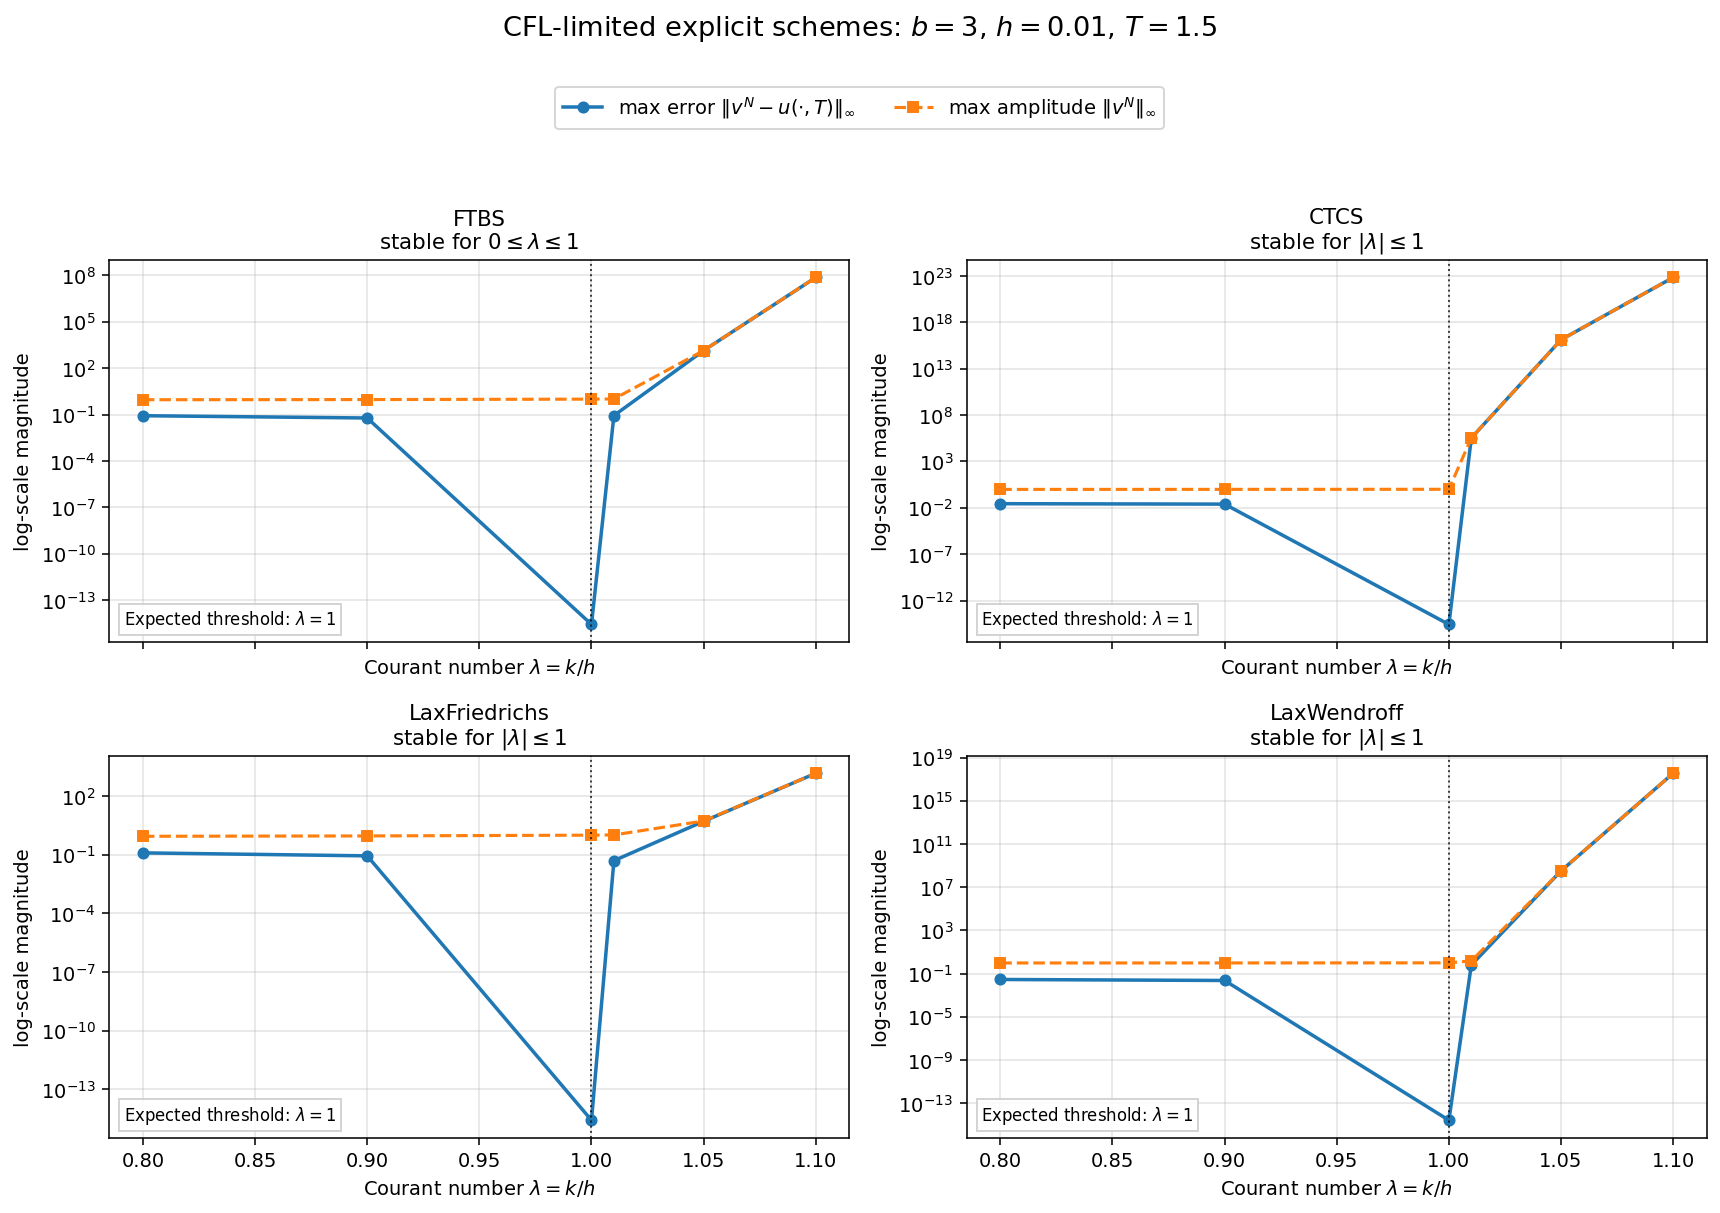
\includegraphics[width=\textwidth]{figures/problem3_lambda_sweep_part1_cfl_limited.png}
    \caption{Sweep in $\lambda$ for explicit schemes with CFL threshold $\lambda=1$.}
\end{figure}

For FTBS, CTCS, Lax--Friedrichs, and Lax--Wendroff, the derived stability condition is
\begin{equation}
    |\lambda|\le 1.
\end{equation}
The plot is consistent with this theory:
\begin{itemize}
    \item For $\lambda=0.8$ and $\lambda=0.9$, the maximum amplitude remains of order
    one.
    \item At $\lambda=1$, several schemes become nearly exact in this special
    experiment because the wave moves exactly one grid cell per time step.
    \item Just above the threshold, such as $\lambda=1.01$, instability may not be
    dramatic over a finite time interval because the unstable amplification factor is
    only slightly larger than one.
    \item For $\lambda=1.05$ and $\lambda=1.1$, the unstable modes have had enough
    growth to become plainly visible, and the maximum amplitude increases rapidly.
\end{itemize}

The near-zero error at $\lambda=1$ should not be interpreted as a general convergence
result.  It is a special grid-alignment effect.  For example, FTBS becomes
\begin{equation}
    v_m^{n+1}=v_{m-1}^n
    \qquad\text{when }\lambda=1,
\end{equation}
which is exactly the grid shift produced by the continuous equation over one time
step.  Similar exact-shift behavior occurs for Lax--Friedrichs and Lax--Wendroff at
$\lambda=1$.

\subsection{Unstable, Wider-Range, and Implicit Methods}

The second split plot groups the methods that do not follow the simple
$|\lambda|\le1$ story.

\begin{figure}[H]
    \centering
    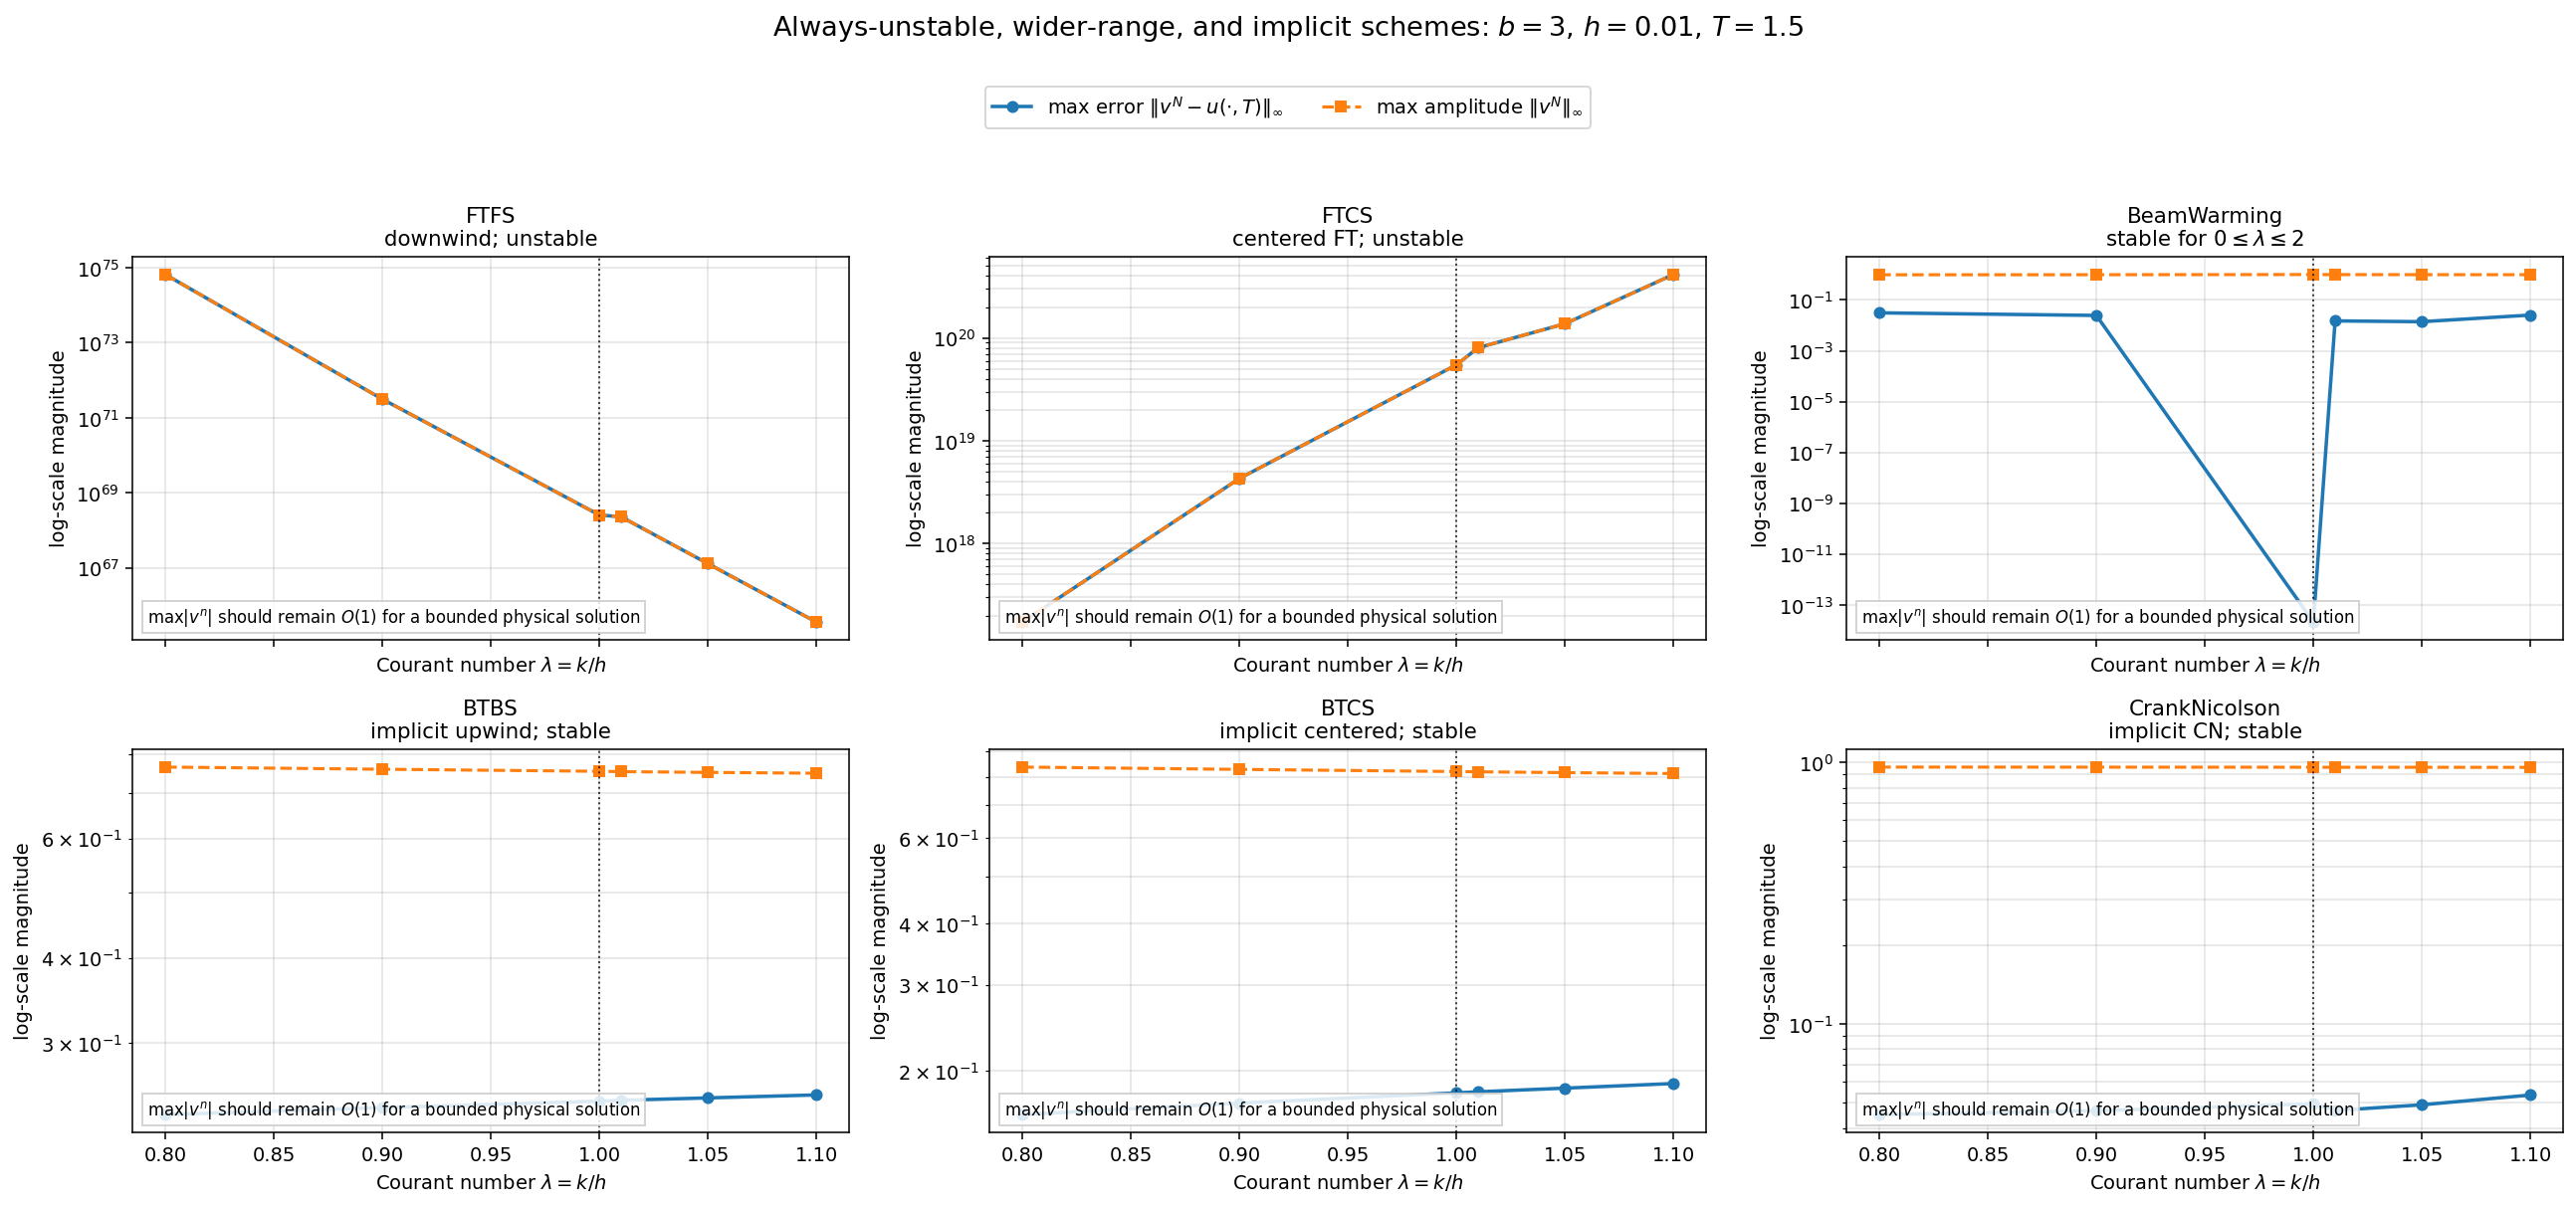
\includegraphics[width=\textwidth]{figures/problem3_lambda_sweep_part2_robust_unstable.png}
    \caption{Sweep in $\lambda$ for always-unstable, wider-range, and implicit schemes.}
\end{figure}

FTFS is unstable because it is the downwind method for the right-moving equation
$u_t+u_x=0$.  Its amplification factor satisfies
\begin{equation}
    |G|^2
    =
    1+2\lambda(1+\lambda)(1-\cos\theta)>1
\end{equation}
for nonzero modes.  Thus reducing $\lambda$ below $1$ does not fix FTFS; the spatial
bias is wrong.

FTCS is also unstable for every nonzero $\lambda$, since
\begin{equation}
    |G|^2=1+\lambda^2\sin^2\theta>1
\end{equation}
for many Fourier modes.  Hence the FTCS curve shows large growth even when
$\lambda=0.8$.

Beam--Warming is stable over the tested range because the theory gives
\begin{equation}
    0\le\lambda\le2.
\end{equation}
The tested values only go up to $\lambda=1.1$, so the method remains bounded in the
sweep.  This does not mean Beam--Warming is always monotone or nonoscillatory; it is a
higher-order upwind method and can still produce dispersive errors near nonsmooth
features.

The implicit methods BTBS, BTCS, and Crank--Nicolson remain bounded as $\lambda$
increases.  Their different behavior is visible in the amplitude:
\begin{itemize}
    \item BTBS is implicit upwind and strongly dissipative, so
    $\norm{v^N}_\infty$ is noticeably below $1$.
    \item BTCS is also stable but still introduces smoothing and phase error.
    \item Crank--Nicolson is neutrally stable, $|G|=1$, so it preserves amplitudes
    better, but it may retain dispersive oscillations near nonsmooth corners.
\end{itemize}

\subsection{Main Conclusion from the Sweep}

The $\lambda$ sweep should be read as numerical evidence for the theoretical
amplification-factor conditions:
\begin{equation}
    \boxed{\text{Stability is controlled by } |G(\theta)|\le1.}
\end{equation}
For CFL-limited explicit schemes, the threshold $\lambda=1$ is visible.  For FTFS and
FTCS, instability occurs even below $\lambda=1$ because their amplification factors
already exceed one.  For Beam--Warming, the wider range $0\le\lambda\le2$ explains why
the method stays bounded beyond $\lambda=1$.  For implicit methods, the absence of a
CFL stability restriction explains why the amplitude remains bounded, although
accuracy and numerical diffusion still depend on $h$ and $k$.

\section{Summary}

\begin{table}[h]
\centering
\begin{tabular}{@{}lll@{}}
\toprule
Scheme & Amplification factor & Stability condition\\
\midrule
FTFS & $1+\nu-\nu e^{\ii\theta}$ & unstable for $\nu>0$\\
FTBS & $1-\nu+\nu e^{-\ii\theta}$ & $0\le\nu\le1$\\
FTCS & $1-\ii\nu\sin\theta$ & unstable for $\nu\ne0$\\
CTCS & $G^2+2\ii\nu\sin\theta\,G-1=0$ & $|\nu|\le1$\\
Lax--Friedrichs & $\cos\theta-\ii\nu\sin\theta$ & $|\nu|\le1$\\
Lax--Wendroff & $1-\ii\nu\sin\theta+\nu^2(\cos\theta-1)$ & $|\nu|\le1$\\
Beam--Warming & second-order upwind symbol & $0\le\nu\le2$\\
BTFS & $(1-\nu+\nu e^{\ii\theta})^{-1}$ & stable for $\nu\ge1$ on a periodic grid\\
BTBS & $(1+\nu-\nu e^{-\ii\theta})^{-1}$ & all $\nu\ge0$\\
BTCS & $(1+\ii\nu\sin\theta)^{-1}$ & all $\nu$\\
Crank--Nicolson & $\dfrac{1-\frac{\ii\nu}{2}\sin\theta}{1+\frac{\ii\nu}{2}\sin\theta}$ & all $\nu$, $|G|=1$\\
\bottomrule
\end{tabular}
\end{table}

\end{document}
